\section{Contexto do estudo}

\begin{frame}{Sistema Inteligente}

\[\boxed{\text{Inteligência artificial} + \text{\alert<2>{Engenharia}} = \text{Sistema Inteligente}}\] 
    
\end{frame}

\begin{frame}{Monitoramento da Integridade Estrutural (SHM)}

\begin{block}{Finalidade}
    Diagnóstico e análise de uma estrutura.
\end{block} \pause

\begin{itemize}
    \item Mecânica
    \item Civil
    \item Aeroespacial/Aeronáutica
\end{itemize} \pause
\vfill
Sensores \(\rightarrow\) Sistema central \(\rightarrow\) Análise dos dados \(\rightarrow\) Decisão
\end{frame}

\begin{frame}{Monitoramento da Integridade Estrutural (SHM)}
Métodos utilizados:

\begin{itemize}
    \item Acelerômetros
    \item Inspeção gráfica \(\rightarrow\) câmeras digitais
    \item \alert<2>{Sensores piezoelétricos}
\end{itemize}

\end{frame}

\begin{frame}{Controle do VANT}
\pause

\begin{block}{O que temos?}
    \begin{itemize}
        \item Algoritmo de controle do VANT.
        \item Implementação em MATLAB.
        \item Trajetórias: retangular, circular e linear.
    \end{itemize}
\end{block} \pause
% \vfill
\begin{figure}
    \centering
    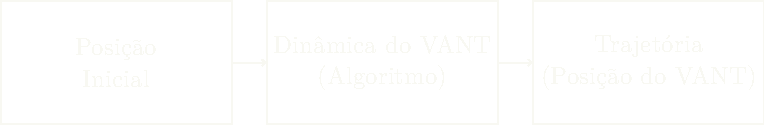
\includegraphics{figures/dinamica_vant.pdf}
    \end{figure}
\end{frame}

\begin{frame}{Controle do VANT}

\begin{block}{O que será feito}
    \begin{itemize}
        \item Algoritmo para determinar as forças usadas.
        \item Dados de entrada: trajetória e posição inicial.
        \item Redes neurais.
    \end{itemize} 
\end{block}
% \vfill
\begin{figure}
\centering
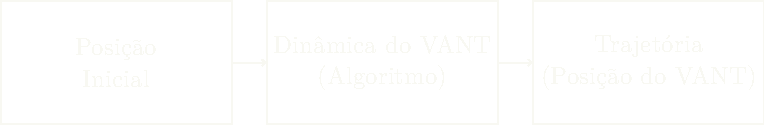
\includegraphics{figures/dinamica_vant.pdf}
\end{figure}
\end{frame}